\documentclass[a4paper]{article}

\usepackage[utf8]{inputenc}
\usepackage[T1]{fontenc}
\usepackage{textcomp}
\usepackage[italian]{babel}
\usepackage{graphicx}
\usepackage{siunitx}
\usepackage{float}
\usepackage{amsmath, amssymb}

\title{Relazione di Laboratorio 3 - Rimbalzi}
\author{Walhout Francesco - Iallorenzi Michele}

\begin{document}
    \maketitle

    \section{Introduzione}
    Una pallina elastica lasciata cadere da un altezza $h_0$ completa un certo numero di 
    rimbalzi, ad intervalli di tempo non costanti, prima di fermarsi.
    La sua energia meccanica varia di un fattore $ \gamma<0$ per ogni rimbalzo,
    per questo possiamo dire che l'altezza massima  $h_n$ raggiunta tra il rimbalzo
    $n$ e il rimbalzo $n+1$ è  data dalla formula:
    \begin{equation}
        \label{eq:altezza 1}
        h_n=h_0 \gamma^{n}
    \end{equation}
    Lo scopo dell'esperienza è quello di studiare il comportamento della pallina a partire
    dalle misure degli istanti di tempo dei rimbalzi, e confrontare le misure con i modelli
    matematici che predicono l'andamento delle altezze e la frequenza dei rimbalzi.

    \subsection{Strumenti utilizzati}
    \begin{itemize}
        \item Una pallina elastica
        \item Uno smartphone o dispostivo di registrazione audio
        \item Un metro a nastro
    \end{itemize}

    \section{Misure ed Analisi}
    \subsection{Misurazione}
    Vogliamo misurare i tempi analizzando una registrazione audio dei rimbalzi della pallina,
    quindi è necessario posizionare lo strumento di registrazione per terra vicino
    a dove faremo cadere la pallina e assicurarsi che l'ambiente sia sufficientemente silenzioso.
    Per poter conoscere il valore di $h_0$, abbiamo utilizzato un metro a nastro per
    fare un segno su un muro ad un altezza conosciuta, e abbiamo poi lasciato cadere
    la pallina dall'altezza del segno, assicurandoci di lasciare spazio a sufficienza per evitare
    che la palla si scontri con il muro o con lo strumento di misurazione.
    Abbiamo registrato il rumore dei rimbalzi della pallina avviando
    la registrazione poco prima di lasciar cadere la pallina e arrestandola subito dopo l'ultimo rimbalzo.
    \begin{figure}[!htb]
        \centering
        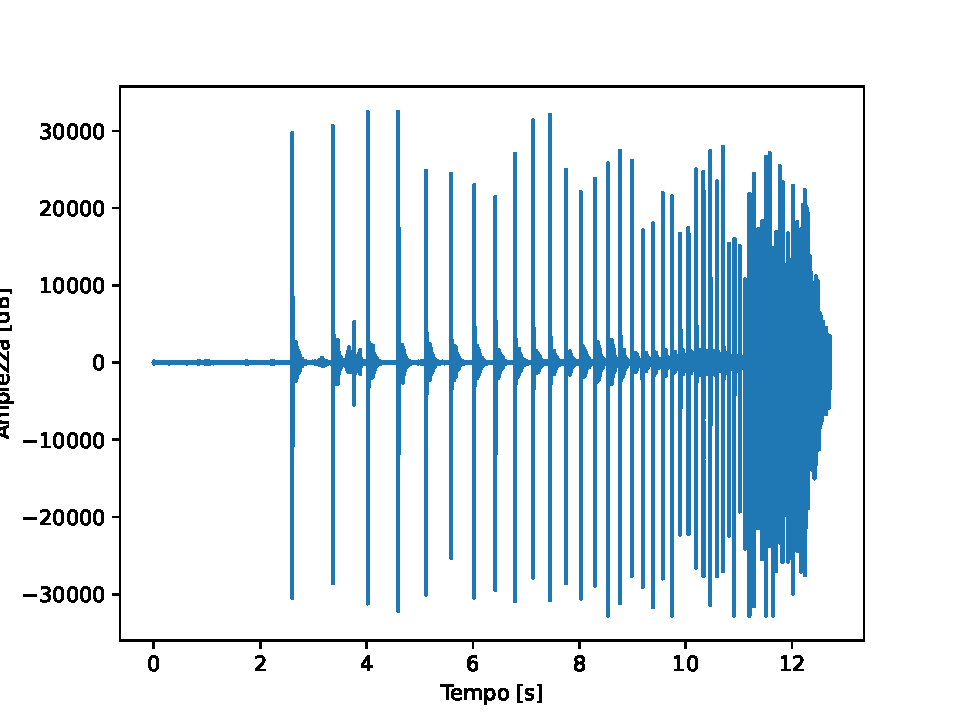
\includegraphics[width=0.8\textwidth]{extra/audio_rimbalzi.pdf}
        \caption{Grafico delle ampiezze della registrazione}
        \label{fig:ampiezze}
    \end{figure}

    \subsection{Campionamento}
    Osservando il grafico delle ampiezze delle registrazioni fatte, si nota che ciascun rimbalzo
    ha un picco iniziale ben definito e una coda più lunga. 
    Abbiamo scelto di campionare come istante di impatto il picco maggiore all'inizio di ciascun rimbalzo,
    ignorando la coda.\\
    Per effettuare il campionamento abbiamo scritto un programma in python che individua
    gli intervalli di tempo in cui l'ampiezza della traccia audio sale sopra ad un threshold
    arbirtrario e per ciascuno restituisce la media dell'istante iniziale e dell'istante finale,
    ovvero l'istante al centro del picco come detto inizialmente.
    I dati così ottenuti sono riassunti nella seguente tabella:\\
    \begin{table}[H]
        \centering
        \begin{tabular}{ll|ll}
            Rimbalzo & Istante [\si{s}] & Rimbalzo & Istante [\si{s}]\\
            \hline
            \hline
            1&4.415&11&9.330\\
            2&5.180&12&9.638\\
            3&5.845&13&9.928\\
            4&6.430&14&10.200\\
            5&6.955&15&10.458\\
            6&7.433&16&10.702\\
            7&7.871&17&10.933\\
            8&8.275&18&11.152\\
            9&8.651&19&11.360\\
            10&9.002&20&11.558
        \end{tabular}
        \caption{Istanti di ciascun rimbalzo della pallina.}
        \label{tab:rimbalzi}
    \end{table}
    \subsection{Elaborazione dei dati}
    Utilizzando le leggi della cinematica per corpi in moto uniformemente accelerato,
    e ignorando quindi l'attrito dell'aria e altre perturbazioni, si può dimostrare la
    seguente formula:
    \begin{equation}
        \label{eq:altezza 2}
        h_n=-\frac{1}{8}g\left( t_n-t_{n-1} \right) 
    \end{equation}
    che ci permette di calcolare le altezze a partire dai dati di cui disponiamo.\\
    Abbiamo quindi fatto un grafico di disperzione di queste altezze ed abiamo fatto il
    fit di questi dati utilizzando funzione curve\_fit di della libreria scipy
\end{document}
